% Fig. 3.20 -- 多對多轉換前後的值域對照 (兩面板)。
% 書稿來源: mathstatch3.tex 第 4484 至 4517 行 (左面板) 與第 4521 至 4552 行 (右面板)，
%   兩個 tikzpicture 各放一個 .48\textwidth 的 minipage 並排，
%   依 CH3_FIGURE_SPECS.md 第二節併為一張兩面板的圖。
% 書稿以 gray、opacity 0.2 填色, 網頁改 journalaccent、透明度 0.15。
%
% 對書稿原圖的三處刻意改正 (比照 Fig. 3.1 的既有處置, 併入勘誤登錄):
%   一、書稿左面板的斜邊自 x=-0.5 畫到 x=3.5、右面板的 z-w=0 自 z=-0.5 畫到 z=3.5，
%       都伸到值域之外甚至座標軸的另一側；網頁把兩條線收在值域範圍之內。
%   二、書稿右面板自 (3,3) 到 (3,0) 的虛線沒有標示，網頁補標 $z=1$，
%       與左面板的 $z=x+y=1$ 相對照。
%   三、書稿在左面板內的 (6,2) 放一個 \xRightarrow，箭號上方的標示含中文「令」；
%       網頁把箭號移到兩面板之間，標示只留 $w=x$ 與 $z=x+y$ 兩式
%       (CH2_FIGURE_SPECS.md 1.4 圖內不得出現中文)。
%
% 字級: 全圖標示一律 \large (12pt)，圖內沒有下標、指數與分數，最小的一級即 12pt。
% 比例尺取 x=y=0.9cm，使原生寬度守在 11.8cm 之內；此圖放在 Note 方框之內，
%   手機顯示寬為 309 px，11.8cm 即 11 px 下限所允許的最大原生寬度。
\documentclass[tikz,border=2pt]{standalone}
\usepackage{amsmath}
\usepackage{amssymb}
\usepackage{xcolor}
\usetikzlibrary{arrows.meta}

\definecolor{journalink}{HTML}{1F1C18}
\definecolor{journalmuted}{HTML}{8A7F72}
\definecolor{journalaccent}{HTML}{9C2D2D}

\begin{document}
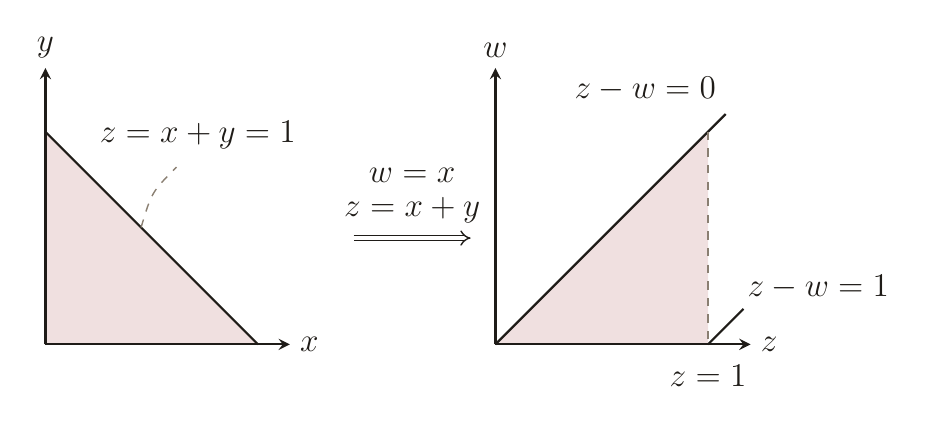
\begin{tikzpicture}[x=0.9cm, y=0.9cm, >=stealth,
                    every node/.style={journalink, font=\large}]

  %% ---- 左面板: 轉換前 (x, y) 的聯合值域 ----
  \begin{scope}[shift={(0,0)}]
    %% 0 < x < 1, 0 < y < 1, x + y < 1 所圍的直角三角形 (圖上 3 個單位即數學上的 1)
    \fill[journalaccent, fill opacity=0.15] (0,0) -- (3,0) -- (0,3) -- cycle;

    %% 斜邊 x + y = 1
    \draw[journalink, line width=0.8pt] (3,0) -- (0,3);

    %% 斜邊的標示與引線
    \node at (2.15,2.95) {$z=x+y=1$};
    \draw[journalmuted, line width=0.5pt, dashed]
      (1.35,1.65) .. controls (1.5,2.15) .. (1.85,2.5);

    %% 座標軸
    \draw[journalink, line width=0.8pt, ->] (0,0) -- (3.45,0) node[right] {$x$};
    \draw[journalink, line width=0.8pt, ->] (0,0) -- (0,3.9) node[above] {$y$};
  \end{scope}

  %% ---- 兩面板之間的轉換箭號 ----
  \begin{scope}[shift={(4.35,0)}]
    \draw[journalink, line width=0.5pt, double, double distance=1.4pt,
          -{Implies[length=5pt]}] (0,1.5) -- (1.65,1.5);
    \node[above, align=center, yshift=2pt] at (0.825,1.5) {$w=x$\\[-0.15em]$z=x+y$};
  \end{scope}

  %% ---- 右面板: 轉換後 (z, w) 的值域 ----
  \begin{scope}[shift={(6.35,0)}]
    %% 0 < w < 1, 0 < z < 1, w < z 所圍的直角三角形
    \fill[journalaccent, fill opacity=0.15] (0,0) -- (3,3) -- (3,0) -- cycle;

    %% 界線 z - w = 0
    \draw[journalink, line width=0.8pt] (0,0) -- (3.25,3.25);
    \node[above left, yshift=1pt] at (3.25,3.25) {$z-w=0$};

    %% 界線 z - w = 1，落在值域之外，並不構成拘束
    \draw[journalink, line width=0.8pt] (3,0) -- (3.5,0.5);
    \node[above right, xshift=-2pt] at (3.5,0.5) {$z-w=1$};

    %% 界線 z = 1
    \draw[journalmuted, line width=0.5pt, dashed] (3,3) -- (3,0);
    \node[below, yshift=-4pt] at (3,0) {$z=1$};

    %% 座標軸
    \draw[journalink, line width=0.8pt, ->] (0,0) -- (3.6,0) node[right] {$z$};
    \draw[journalink, line width=0.8pt, ->] (0,0) -- (0,3.9) node[above] {$w$};
  \end{scope}

\end{tikzpicture}
\end{document}
